
%(BEGIN_QUESTION)
% Copyright 2010, Tony R. Kuphaldt, released under the Creative Commons Attribution License (v 1.0)
% This means you may do almost anything with this work of mine, so long as you give me proper credit

Sketch a waveform showing the hexadecimal value {\tt 5C} sent in NRZ-encoded serial form, complete with start bit, stop bit, an ``odd'' parity bit, and all eight bits of the data sent in proper order.

\vfil

\underbar{file i02224}
\eject
%(END_QUESTION)





%(BEGIN_ANSWER)

This is a graded question -- no answers or hints given!

%(END_ANSWER)





%(BEGIN_NOTES)

$$\includegraphics[width=15.5cm]{i02224x01.eps}$$

Note how the value of the parity bit is ``1'' because there are four ``1'' bits in the data portion, which would be an even number of 1's if not for the parity bit.

%INDEX% Networking, serial data: asynchronous data format
%INDEX% Networking, serial data: start bit
%INDEX% Networking, serial data: stop bit

%(END_NOTES)


